\documentclass[11pt,twocolumn]{article}

\usepackage{epsfig}
\usepackage{graphicx}
\usepackage{graphpap}
\usepackage{amsmath}
\usepackage[latin1]{inputenc}
\usepackage[spanish]{babel}

\topmargin -2.5 cm
\textheight 9.5in
\oddsidemargin -1cm
%\evensidemargin -1cm
\textwidth 18cm

\title{}
\author{}
\date{}

\newcommand{\abre}{\textquestiondown}

\begin{document}
\pagestyle{empty}
\sffamily
\twocolumn[

F�sica de Campos. TALLER 5: \textbf{LEY DE GAUSS }

\hrulefill 
\vspace{0.3 cm}
]

\footnote{Las figuras han sido tomadas en su gran mayoria de Physics For Scientist and Engineers 6E By Serway and Jewett}

\begin{enumerate}

%ejercicio
\item (Problema conceptual) Use la ley de Gauss para calcular el campo el�ctrico de una carga puntual $Q$. 
{
\begin{center}
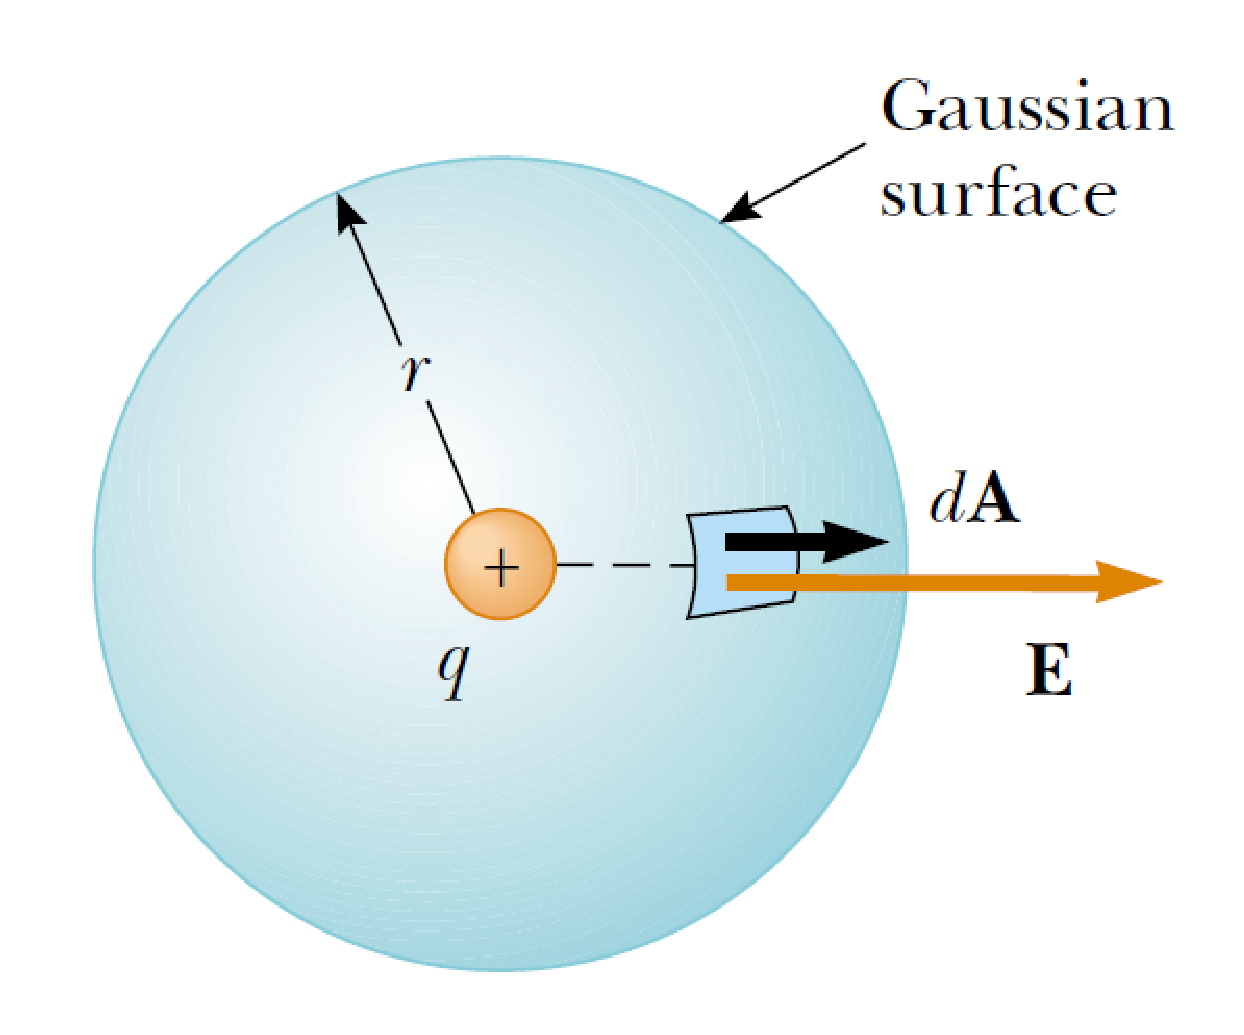
\includegraphics[scale=0.2]{carga-puntual}
\end{center}
}
\begin{displaymath}
\vec{E}=k\dfrac{Q}{r^2}\hat{u_{r}}
\end{displaymath}

%ejercicio
\item Use la ley de Gauss para calcular el campo de una esfera aislante de radio $a$ de carga $Q$ distribuida uniformemente. 
{
\begin{center}
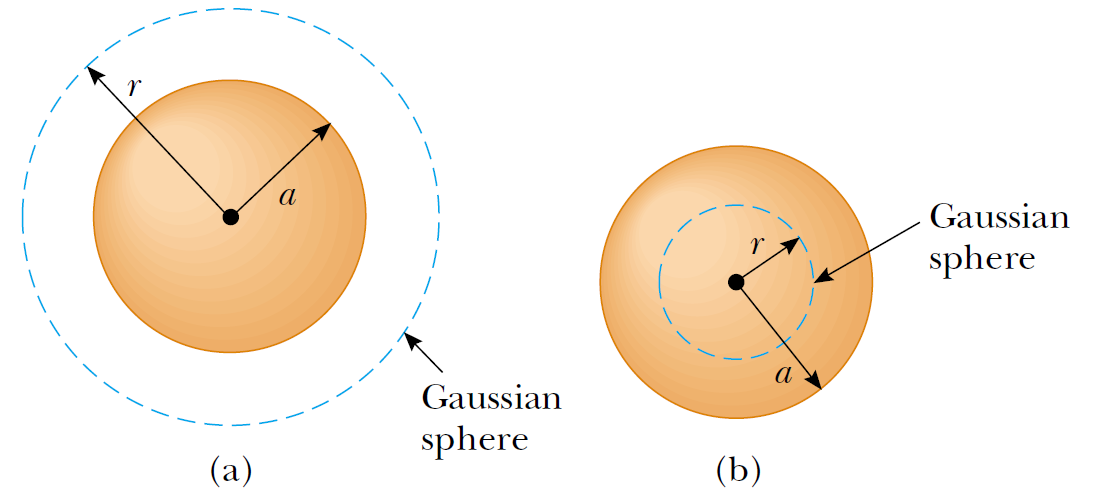
\includegraphics[scale=0.2]{esfera-gauss}
\end{center}
}
\begin{displaymath}
\vec{E}=k\dfrac{Q}{r^2}\hat{u_{r}} \hspace{0.2 cm} (r \geq a) \hspace{0.6 cm} \vec{E}=k\dfrac{Q r}{a^3}\hat{u_{r}} \hspace{0.2 cm} (r \leq a).
\end{displaymath}

%ejercicio
\item Use la ley de Gauss para calcular el campo de una esfera \textit{conductora} de radio $a$ de carga $Q$. 
{
\begin{center}
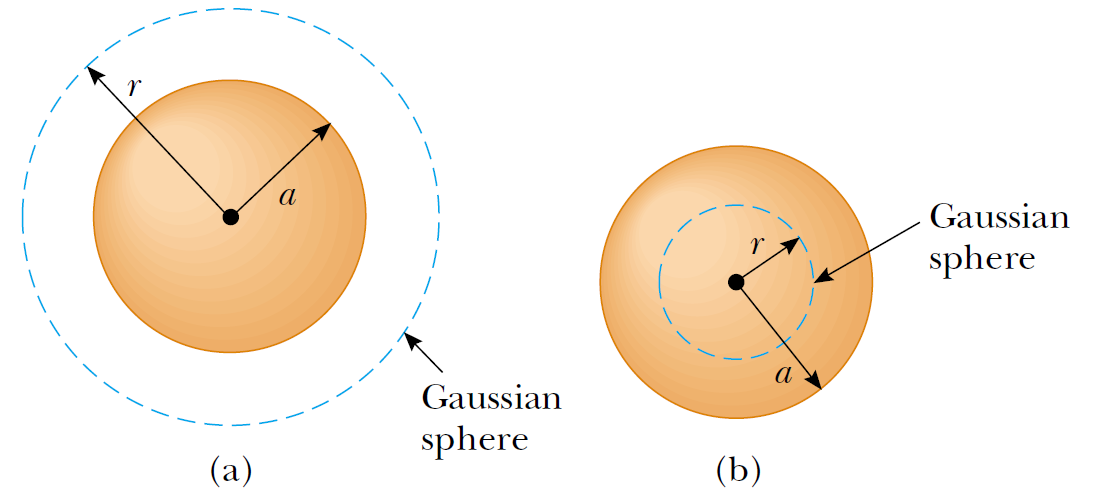
\includegraphics[scale=0.2]{esfera-gauss}
\end{center}
}
\begin{displaymath}
\vec{E}=k\dfrac{Q}{r^2}\hat{u_{r}} \hspace{0.2 cm} (r\geq a) \hspace{0.6 cm} E=0 \hspace{0.2 cm} (r\leq a).
\end{displaymath}


%ejercicio
\item Calcule el campo el�ctrico de una varilla infinita de densidad de carga $\lambda$.
\begin{displaymath}
\vec{E}=\dfrac{2k\lambda}{r}\hat{u_{r}}
\end{displaymath}
{
\begin{center}
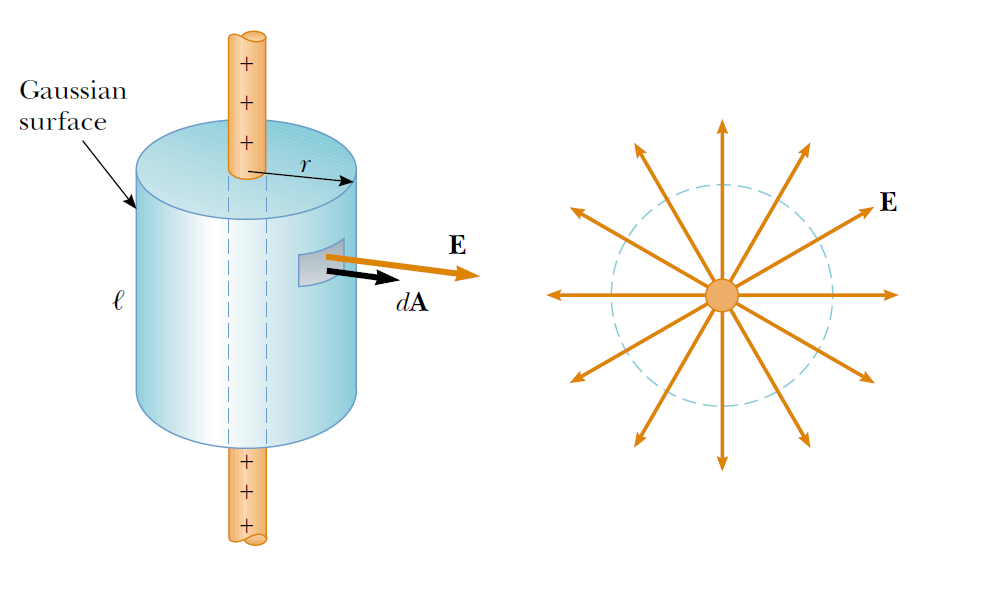
\includegraphics[scale=0.2]{alambre-gauss}
\end{center}
}

%ejercicio
\item Calcule el campo el�ctrico de un plano infinito de densidad de carga superficial $\sigma$.
\begin{displaymath}
\vec{E}=\dfrac{\sigma}{2\epsilon_{0}}\hat{k} 
\end{displaymath}
{
\begin{center}
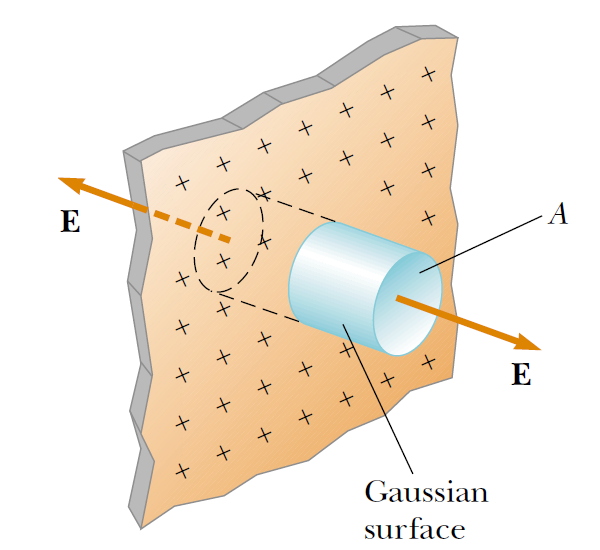
\includegraphics[scale=0.25]{plano-gauss}
\end{center}
}

%ejercicio
\item Calcule el campo el�ctrico de un par de placas paralelas (infinitas) de densidad de carga $\sigma$ y $-\sigma$.
{
\begin{center}
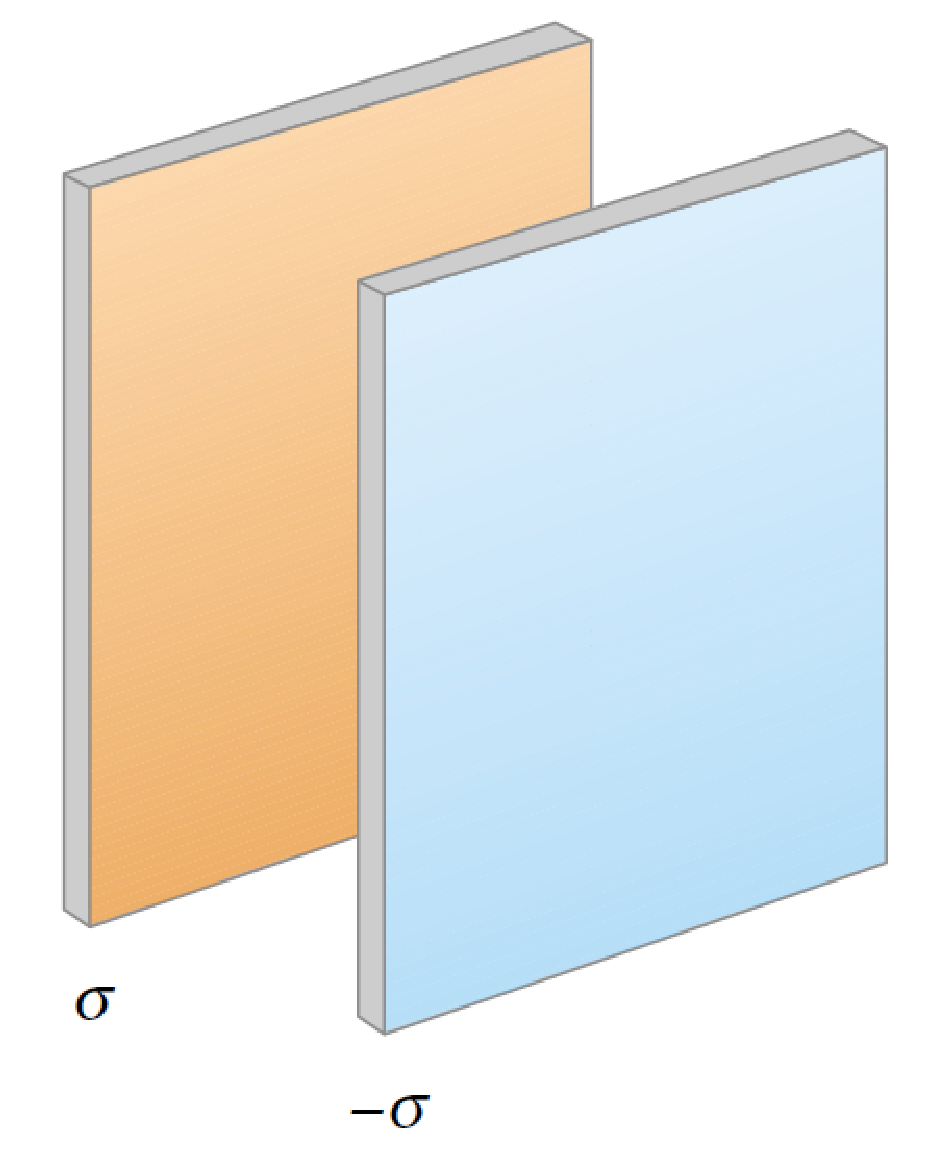
\includegraphics[scale=0.2]{placas-paralelas}
\end{center}
}
\begin{displaymath}
E=\dfrac{\sigma}{\epsilon_{0}} \hspace{0.3 cm} (interior) \hspace{0.3 cm} E=0 \hspace{0.3 cm} (exterior)
\end{displaymath}

%ejercicio
 \item Una esfera conductora de radio $a$ tiene una carga neta $2Q$. Un cascar�n esf�rico conductor de radio interior $b$ y radio exterior $c$ es conc�ntrica con la esfera y lleva una carga neta $-Q$. Halle el campo el�ctrico en las regiones $1,2,3,4$. �C�mo es la distribuci�n de carga sobre ambos conductores?	
{
\begin{center}
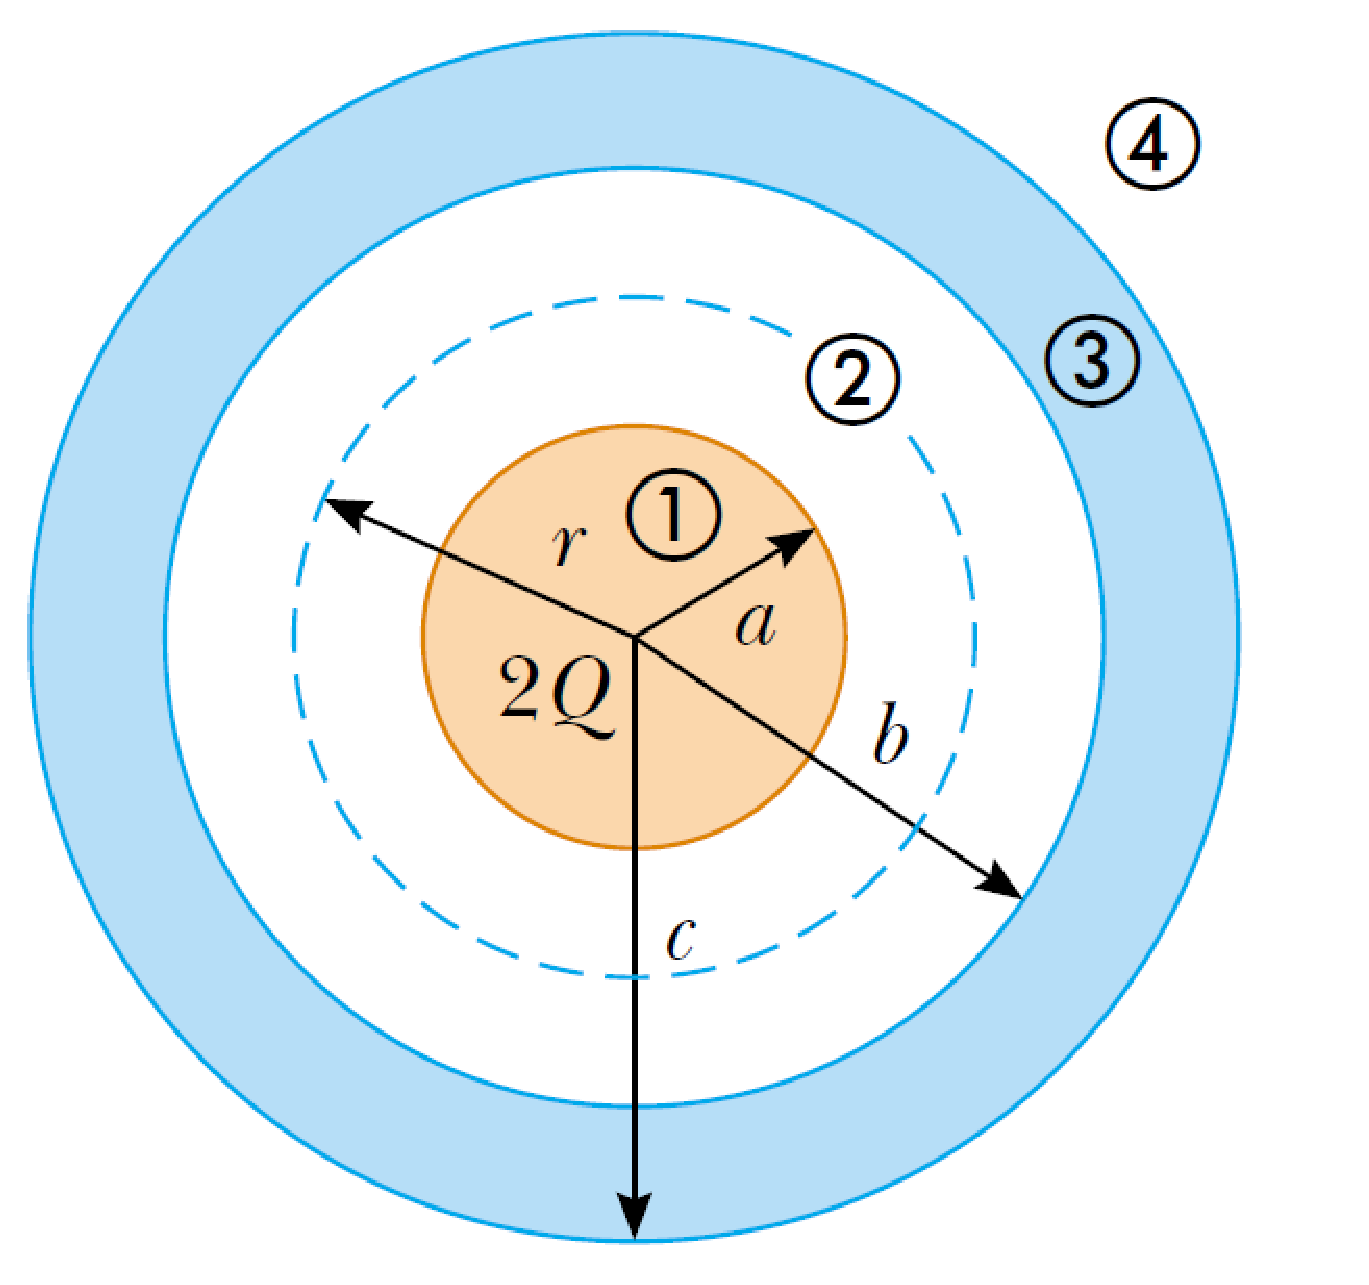
\includegraphics[scale=0.2]{esfera-conductor}
\end{center}
}

%ejercicio
\item Una esfera de radio $R$ encierra una carga puntual $Q$ localizada en su centro. 
\begin{enumerate}
\item Muestre que el flujo est� dado por la siguiente expresi�n:
\begin{displaymath}
\Phi_{E}=\dfrac{Q}{2\epsilon_{0}}(1-\cos{\theta})
\end{displaymath}
{
\begin{center}
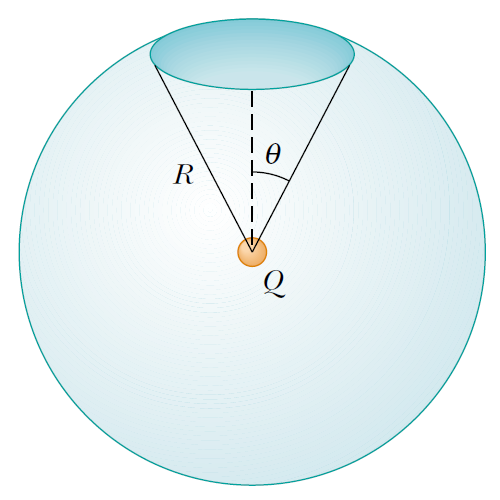
\includegraphics[scale=0.25]{flujo-gauss}
\end{center}
}
\item Halle el flujo para $\theta=90�$ y $\theta=180�$.
\end{enumerate}

\item Una cascar�n esf�rico de radio exterior $R_{1}$ y radio interior $R_{2}$ tiene una densidad de carga $\rho=\tilde{k}/r$. En el centro del cascar�n esf�rico se tiene una carga puntual $-q$. Halle el campo el�ctrico para $r<R_{2}$ , $R_{2}<r<R_{1}$ y $r>R_{1}$.  
\begin{displaymath}
\vec{E}=-\dfrac{kq}{r^2}\hat{u_{r}} \hspace{0.5 cm} (r<R_{2})
\end{displaymath}
\begin{displaymath}
\vec{E}=\dfrac{k}{r^2}\Big[2\pi\tilde{k}(r^2 -R_{2}^2)-q\Big]\hat{u_{r}} \hspace{0.5 cm} R_{2}<r<R_{1}
\end{displaymath}
\begin{displaymath}
\tilde{k}=\dfrac{1}{2\pi(R_{1}^2 -R_{2}^2)}
\end{displaymath}
\begin{displaymath}
\vec{E}=k\dfrac{Q-q}{r^2}\hat{u_{r}} \hspace{0.5 cm} (r>R_{1}).
\end{displaymath}

%ejercicio
\item Una esfera conductora s�lida de radio $R_{1}$ tiene una carga positiva neta de $3Q$. Un cascar�n esf�rico conductor de radio interior $R_{2}>R_{1}$ y radio exterior $R_{3}$ es conc�ntrico con la esfera s�lida y tiene una carga neta de $-Q$. Halle el campo el�ctrico para $r<R_{1}$, $R_{1}<r<R_{2}$, $R_{2}<r<R_{3}$, y $r>R_{3}$. 
\begin{displaymath}
E=0 \hspace{0.5 cm} (r<R_{1}), \hspace{0.5 cm} \vec{E}=k\dfrac{3Q}{r^2}\hat{u_{r}} \hspace{0.5 cm} R_{1}<r<R_{2}
\end{displaymath}
\begin{displaymath}
E=0 \hspace{0.5 cm} R_{2}<r<R_{3}
\end{displaymath}
\begin{displaymath}
\vec{E}=k\dfrac{2Q}{r^2}\hat{u_{r}} \hspace{0.5 cm} r>R_{3}
\end{displaymath}

%ejercico
\item Calcule el campo de un cil�ndro macizo de largo $l$ grande (infinito) y radio $R$ usando la ley de Gauss. Calculelo para $r<R$ y $r>R$.

\item Un Cil�ndro conductor de radio $a$ y carga $Q$ es coaxial con un cascar�n cil�ndrico de grosor despreciable, radio $b>a$, y carga $-Q$. Halle el campo el�ctrico para $r<a$, $a<r<b$, y $r>b$.
\begin{displaymath}
\vec{E}=\dfrac{\lambda}{2\pi\epsilon_{0}}\hat{u_{r}} \hspace{0.5 cm} (a<r<b).
\end{displaymath}
{
\begin{center}
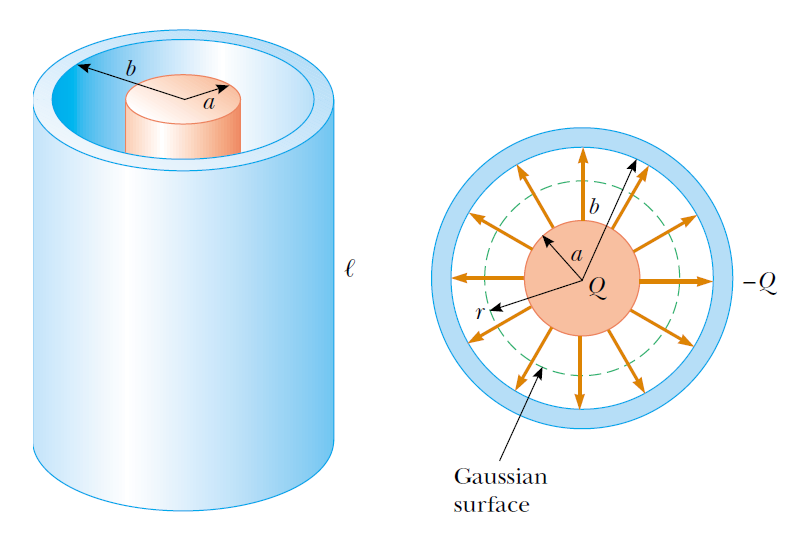
\includegraphics[scale=0.25]{cilindro-gauss}
\end{center}
}



\end{enumerate}
\end{document}
